
\documentclass{vldb}
\usepackage{graphicx}
\usepackage{balance}

% \usepackage{amsmath}
\usepackage[noend]{algpseudocode}
\usepackage{algorithm}
% \usepackage{xspace}

\algnewcommand\Label[1]{\item[#1:]}

\begin{document}

\title{Let vehicles work together:
Towards the next generation of city transportation schedule}

\numberofauthors{1}
\author{
\alignauthor
Hebi Li\\
       \affaddr{Iowa State University}\\
       \affaddr{4300 Westbrook Dr}\\
       \affaddr{Ames, Iowa}\\
       \email{hebi@iastate.edu}
}

\maketitle

\begin{abstract}
We explore the scenario that, in the future, no one's going to drive a car.
Driverless cars are running inside the city to take people from place to place.
How to efficiently schedule these auto-drive vehicles to reach overall the most efficiency?
In this paper, we give the first definition of this problem.
We propose a complete schedule algorithm to make these new format of taxis work together to reach the efficiency requirement.
Also, we propose the Segmented RTree to solve the key challenge in the proposed schedule algorithm,
which is a general method of a category of problems.
The extensive experiments we did on both simulation data and actual data from google map
shows that our solution does a great job compared to naive solution,
and segmented RTree overperforms the state-of-the-art query index algorithm for this category of problem.
\end{abstract}




\section{Introduction}

We believe that driverless cars will eventually substitute the main transportation method,
private cars, in the future.
First, it is safer to take a driverless car than driving manually,
because computer is highly reliable, and will stay focused 24x7,
while people are often tired, attracted by other things, or even drunk when driving a car.
Google’s driverless cars have been extensively experimented and proved to be extremely safe.
People are doing research such as artificial intellegence to make the algorithm even better and better.
Second, it is cheaper for people to just take cars instead of buying vehicles for their own use.
As in a survey, every family in America has averagely 2.5 cars parked in their lot.
Besides, it is more convenient, because you can take the cars at any time from anyplace,
no need to carry your car everywhere you go. What’s more, it is more environment friendly.
People who have overlapped trajectory can share a car.
It can save much energy and reduce pollution.

In this scenario, people will have no need to own a car and drive theirselves.
There're hundreds of thoudsands of cars on the street.
When people need a travel, he just need to submit his request to the \textit{central control system},
containing when he wants to be picked up, from where to where,
and other requirements such as the arriving time period,
how many times he can endure to exchange car, does he allow sharing cars with others, etc.
Upon receiving this request,
the central control system should come out a complete schedule for the cars to complete this travel.

While the transportation schedule problem was studied extensively in the past,
they mainly focus on the shortest path from location to location,
salesman problem to go through every cities exactly once at the least cost, weighted route.
But for our problem,
we are focusing on how to schedule hundreds of thousands of cars efficiently for
potentially very large amount of user requests.
Besides, we consider that cars can be shared by people who have overlapped trajectory.
What's more, in our scenario, we consider that people can be dropped off in the middle of the trip,
and be picked up by another vehicle to reach the most efficiency of the whole system.
People are incentive to do this because this can reduce the cost he need to pay for the trip.
This senario is like a super public transportation system,
but is much more powerful than it.
Bus or subway has predefined route, predefined interval,
thus is essentially a small subset of the considered scenario.

It is non-trival because both vehicle number and user request number can be very large.
A naive solution could be that, for every user request, find the nearest free car to take him to the destination.
The total distance of cars movement is roughly the same as people just drive their own cars to the destination.
What’s more, It is difficult to find a car near a place at a specific time,
not to say that we have hundreds of thousands of cars to be selected,
and user requests are huge. People usually needs to get the schedule immediately,
since the best car for him to use may be just 5 seconds away from him, and will pass away quickly.
So it is highly required to work out the schedule efficiently.

The critical problem in our schedule algorithm is
how to predict which cars are near a specific location at a specific time.
Existing solution cannot handle it very well.
Spacial Index method such as RTree can not handle it because cars are constantly moving at their own trajectory,
which is highly polynomial and can be changed.
TP-Rtree reach bad efficiency. In this paper, We propose Segmented RTree to solve it efficiently.

We should notice that, in spite that driverless cars in the future are our motivation to do this research,
our problem also fits in many other applications where need similar schedule.
For example, for a big taxi company who has a lot of vehicles nowadays,
they can provide this service to customer for their convenience at a appealing low price.
Also, for indexing spatial moving objects,
our proposed segmented RTree solve an important sub problem
by adding a common assumption that location of an object is continuous and cannot change too rapidly.

Our contributions are concluded as follows:
\begin{itemize}
  \item we proposed the first definition of the problem of scheduling vehicles to reach overall efficiency(\$\ref{definition}).
  \item we proposed an efficient algorithm towards the solution to the problem(\$\ref{schedule}).
  \item we proposed segmented RTree to tackle the critical problem in the schedule algorithm
  to efficiently retrieve the item list in a specific region at a specific time(\$\ref{segmented_rtree}).
  \item we implemented the proposed solution and experimented extensively,
  and it proved to be efficient and useful(\$\ref{implementation}).
\end{itemize}

% The following is organized as follows.
% Related work are summerized in Section \ref{related_work}.
% We provide problem definition and our assumptions in Section \ref{preliminary}.
% In Section \ref{schedule}, we discuss the proposed schedule algorithm,
% and we talk about the Segmented RTree in Section \ref{segmented_rtree}.
% Implementation and evaluation are given in Section \ref{implementation}.
% We discuss some interesting topics related to this paper in Section \ref{discussion}.
% Finally, we conclude our paper and provide future work in Section \ref{conclusion}.



\section{Preliminary}
\label{definition}
\subsection{problem definition}
There is a central control system that accepts users' queries and schedule vehicles to pick them up.
The central control system knows all vehicles' information, including their locations,
current passengers they are carrying,
as well as their current trajectories.
The central server accepts user request, so it knows the information about all users.
For example, the take off time of the user, the source and destination,
as well as other requirements like the arrival time period,
willing to share the car with anyone else or not,
as well as how many times can he/she endure to transfer a car.

On output, the central control system should work out a \textit{complete schedule}
which make the whole system efficient while satisfies everyone's specific requirements.
By the whole system efficiency,
we mean that the schedule should minimize the total running distance of all vehicles.

\subsection{assumption}
We assume control center knows info about every car.
This includes its locations,
current passengers and their destinations and requirements,
and its current trajectory.
Further, we assume that according to a (src, dest) pair,
control center can come out the best trajectory (with consideration of traffic jam, highway, etc).
This can be done by query a service such as google map, so its no need to reinvent a wheel.

The most important assumption come out to be that,
vehicles move continously, and have a limited speed.
In other words, cars cannot jump to another place.
For example, cars cannot reach a 1000 miles per hour speed.

\section{Proposed Schedule Algorithm}
\label{schedule}

In this section, we propose our schedule algorithm that meets the whole system efficiency requirement.

% \begin{algorithm}
%   \caption{Test}
%   \begin{algorithmic}[1] % every 1 line will be numbered
%     \Procedure{MyProcedure}{}
%     \State $\textit{stringlen} \leftarrow \text{length of } \textit{string}$
%     \State $i \leftarrow \textit{patlen}$
%     % \BState \emph{top}:
%     \If {$i > \textit{stringlen}$} \Return false
%     \EndIf
%     \State $j \leftarrow \textit{patlen}$
%     \emph{loop}:
%     \If {$\textit{string}(i) = \textit{path}(j)$}
%     \State $j \leftarrow j-1$.
%     \State $i \leftarrow i-1$.
%     \State \textbf{goto} \emph{loop}.
%     \State \textbf{close};
%     \EndIf
%     \State $i \leftarrow i+\max(\textit{delta}_1(\textit{string}(i)), \textit{delta}_2(j))$.
%     \State \textbf{goto} \emph{top}.
%     \EndProcedure
%   \end{algorithmic}
% \end{algorithm}

\begin{algorithm}
  \caption{Schedule Algorithm}
  \label{schedule_algorithm}
  \begin{algorithmic}[1] % every 1 line will be numbered
    \Procedure{Schedule}{}
      \State $\textit{(time, src, dest, requirements)} \leftarrow \text{user request}$
      \Label \text{loop:}
      \State $\textit{vehicles} \leftarrow \text{GetVehicleList(time, src)}$
      \State $\textbf{filter } \textit{vehicles}$
      \For{$\textit{vehicle} \textbf{ in } \textit{vehicles}$}
        \State $\textit{trojectory} \leftarrow \textit{QueryTrajectory(vehicle)}$
        \State $\textit{(time, loc)} \leftarrow \textit{GetDropoffPoint(trajecotry, dest)}$
        \State $\textit{droppoints}.append \textit{(time, loc)}$
      \EndFor
      \State $\textit{(time, loc)} \leftarrow \textit{SelectClosest(droppoints)}$
      \If{$\textit{loc} = \textit{dest}$} \Return
      \Else
        \State $\textit{time, src} \leftarrow \textit{time, loc}$
        \State \textbf{goto} \emph{loop}
      \EndIf
    \EndProcedure
  \end{algorithmic}
\end{algorithm}

The schedule algorithm is shown in Algorithm \ref{schedule_algorithm}.
On receiving an user request,
the central control system extracts the tuple $(time, src, dest, requirements)$.
Then it executes the procedure \textit{GetVehicleList(time, location)}
to find the vehicles list near the customer at his leaving time.
The system filters the returned vehicle list according to user's specific requirements,
the vehicle's capacity, the vehicle's current trajectory direction,
the passengers' requirements, etc.

For every vehicle in the filtered vehicle list,
compute the dropoff point for this customer if he takes this car,
and add the time and location of the drop point to a list of droppoints.
The system select the closest drop points from all possible ones.
Whenever the drop point reach the final destination, the system output the desired schedule,
otherwise, it repeat this step with the start point and time substituted as the closest drop point
(i.e. the returned \textit{(time, loc)} pair).

\begin{figure}[ht!]
  \centering
  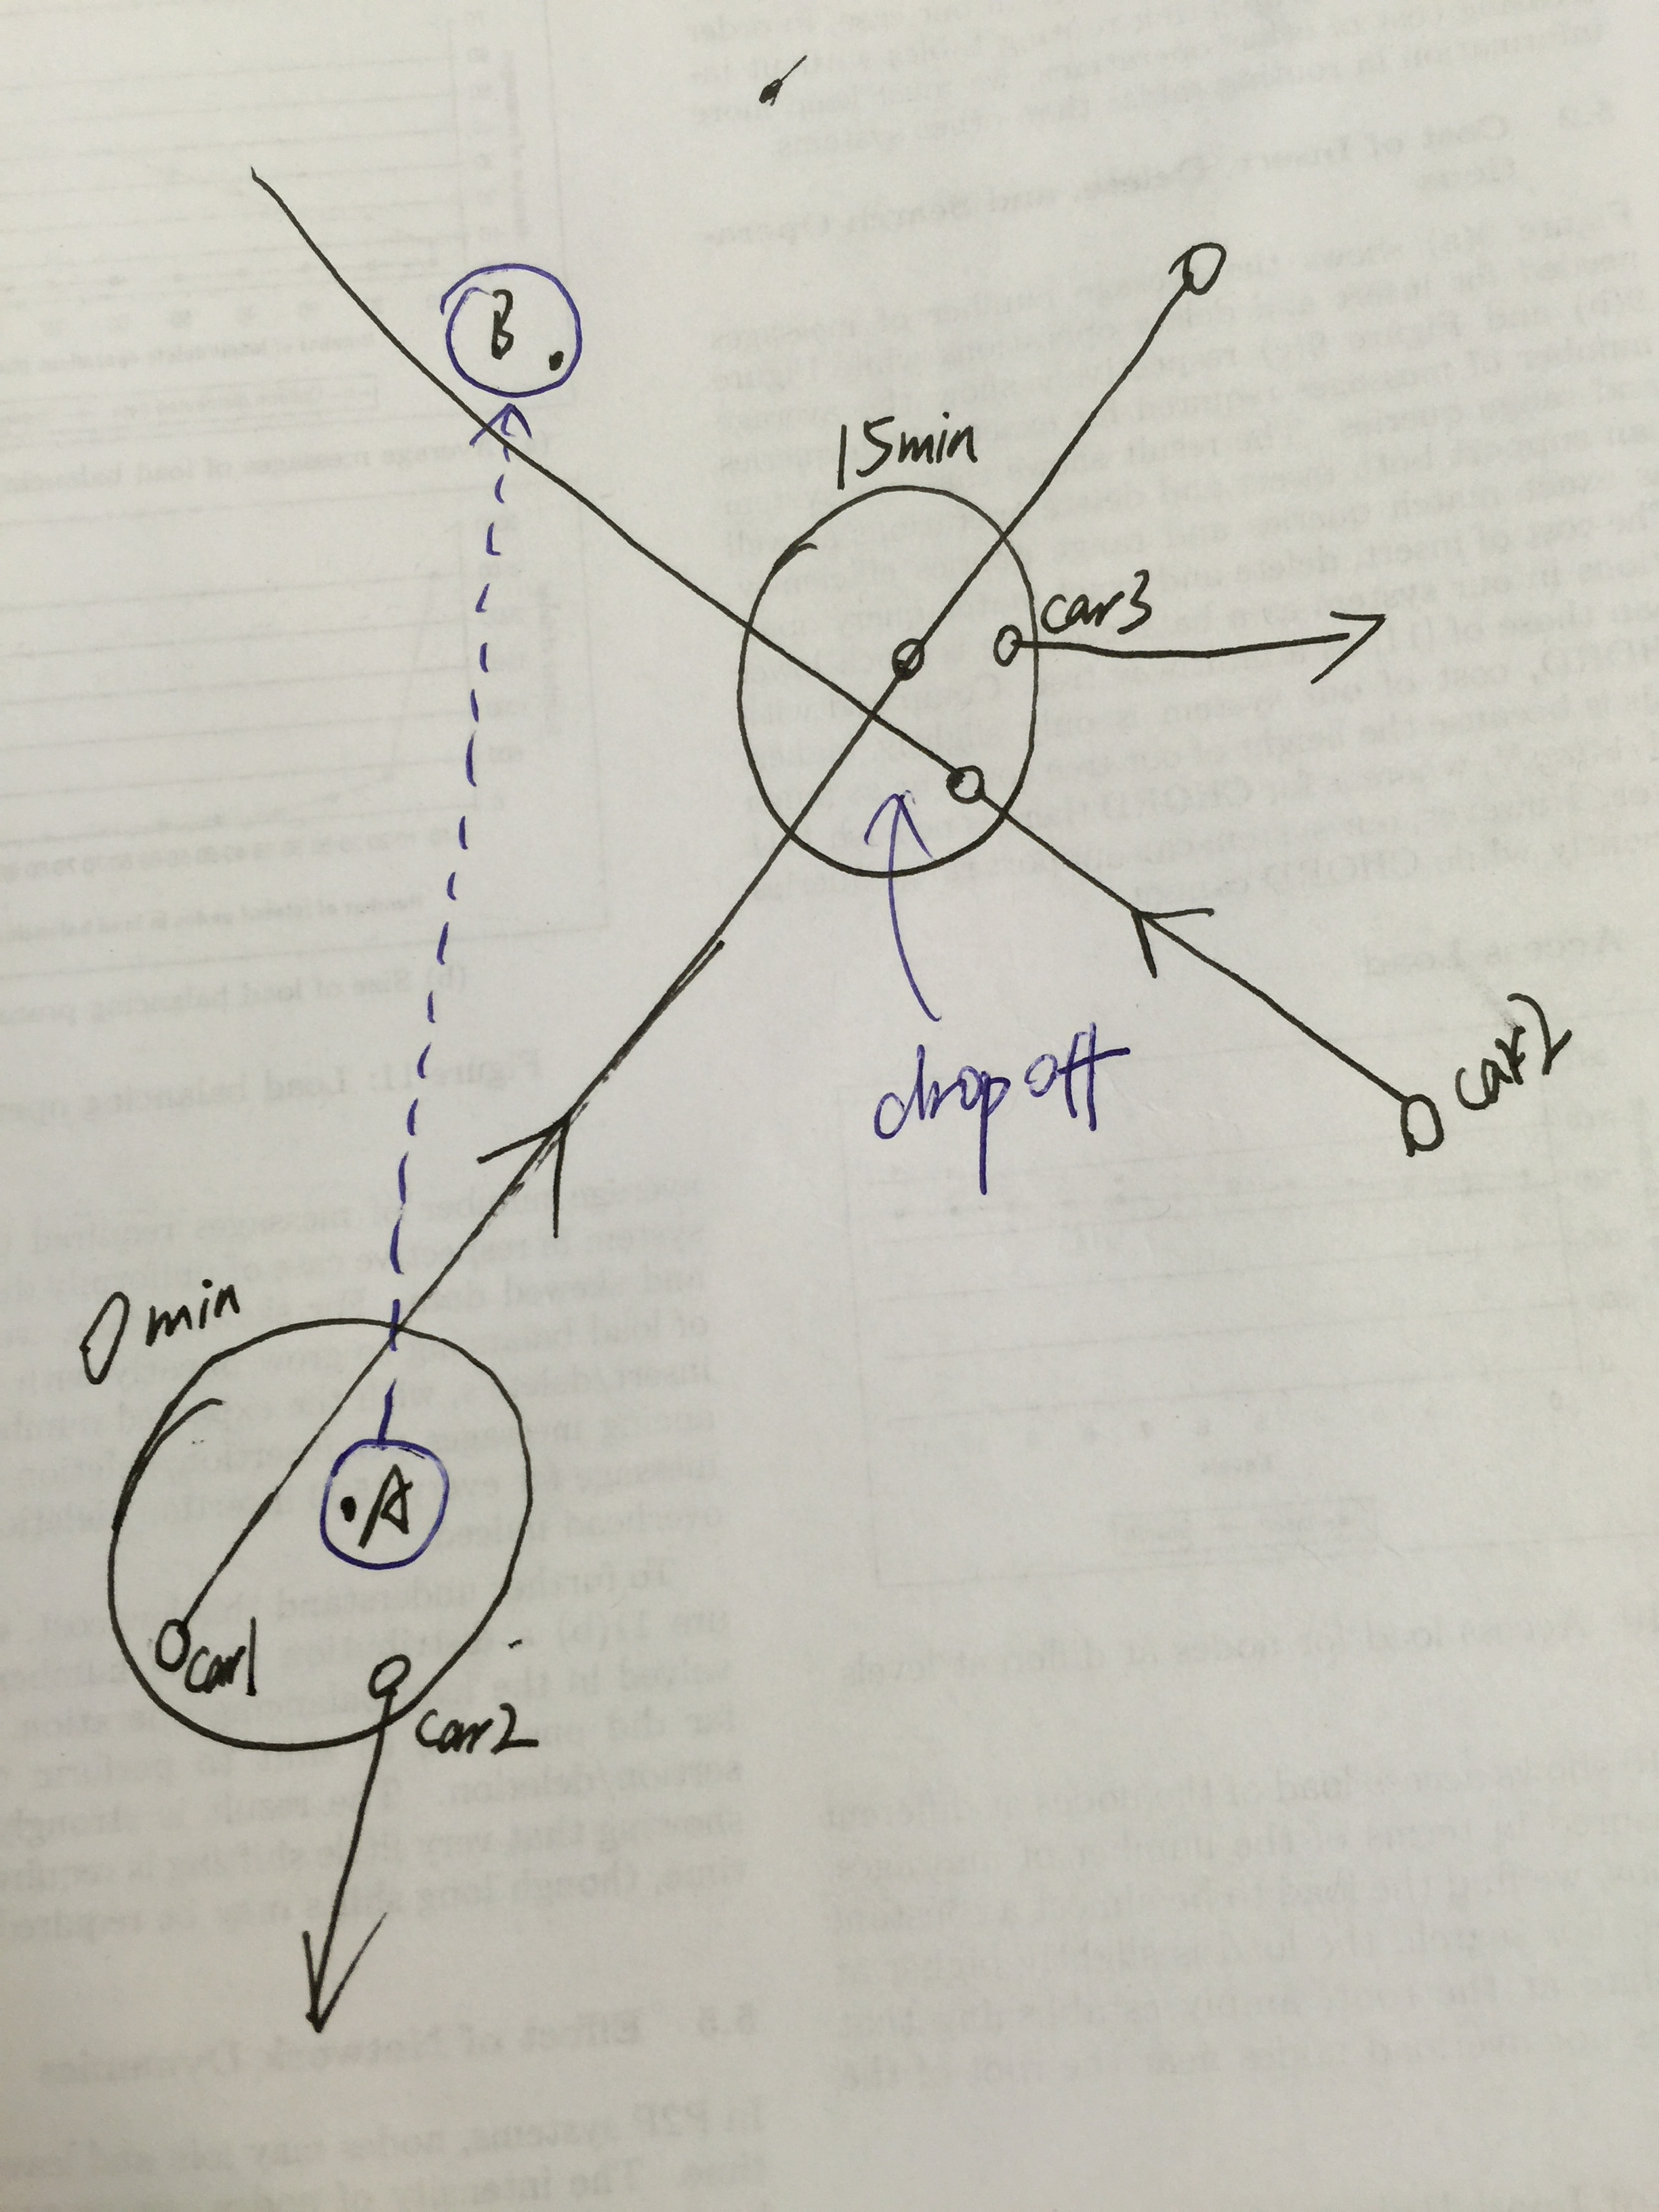
\includegraphics[width=90mm]{schedule.jpg}
  \caption{Schedule Example \label{schedule_fig}}
\end{figure}

As an example, in figure \ref{schedule_fig}. %TODO

How to filter through the vehicle list is out of the scope of this paper.
Some simple yet practical solution is to look at the trajectory and direction,
and filter out the cars that go to a different direction.
User requirements includes how many times he is willing to transfer,
the expected time to arrive,
whether he is willing to share a car with others.
The system can use these information to further filter the vehicles,
but the detail of how to do this is not our focus.

As our assumption, the procedure \textit{QueryTrajectory(vehicle)} is possible
because the system can get trajecotry information for each vehicle.
The procedure \textit{GetDropoffPoint(trajectory, dest)} can be done
by simply calculate the point on the trajecoty that is nearmost the destination.
Intuitively, this procedure can perform better if we take the time into consideration.
For example, if vehicle A can reach a point $Loc_1$ that is 5 miles from the destination in 5 minutes,
but will go on to a round trip and finally reach a place $Loc_2$ that is 4 miles from destination in 20 minutes,
the procedure should probably select $Loc_1$ as the best choice of dropping off.
What's more, the procedure may return a list of possible dropoff points and time for the system to choose from.
How to furthur optimize drop-off point is not our focus in this paper.

The key difficult is thus falling into how to implement the procedure \textit{GetVehicleList(time, loc)}.
In other words, the key problem of the schedule algorithm is
how to efficiently find vehicles near a location in a specific time period.
This problem is chanllenging because both vehicles number and users requrests are huge,
thus it is impossible to simply loop through all vehicles to see if it is near the location at the given time.
Existing solutions to index spactial objects and moving objects can not handle this scenario very well.
We proposed a variant of RTree, the Segmented RTree, which is carefully designed to suit this catagory of scenarios.

\section{Segmented RTree}
\label{segmented_rtree}
In this section, we propose the Segmented RTree to solve the key problem of our schedule algorithm.
We first formally define the problem, give the assumptions, and then propose the design.
\subsection{Formalization and Assumptions}

\begin{figure}[ht!]
  \centering
  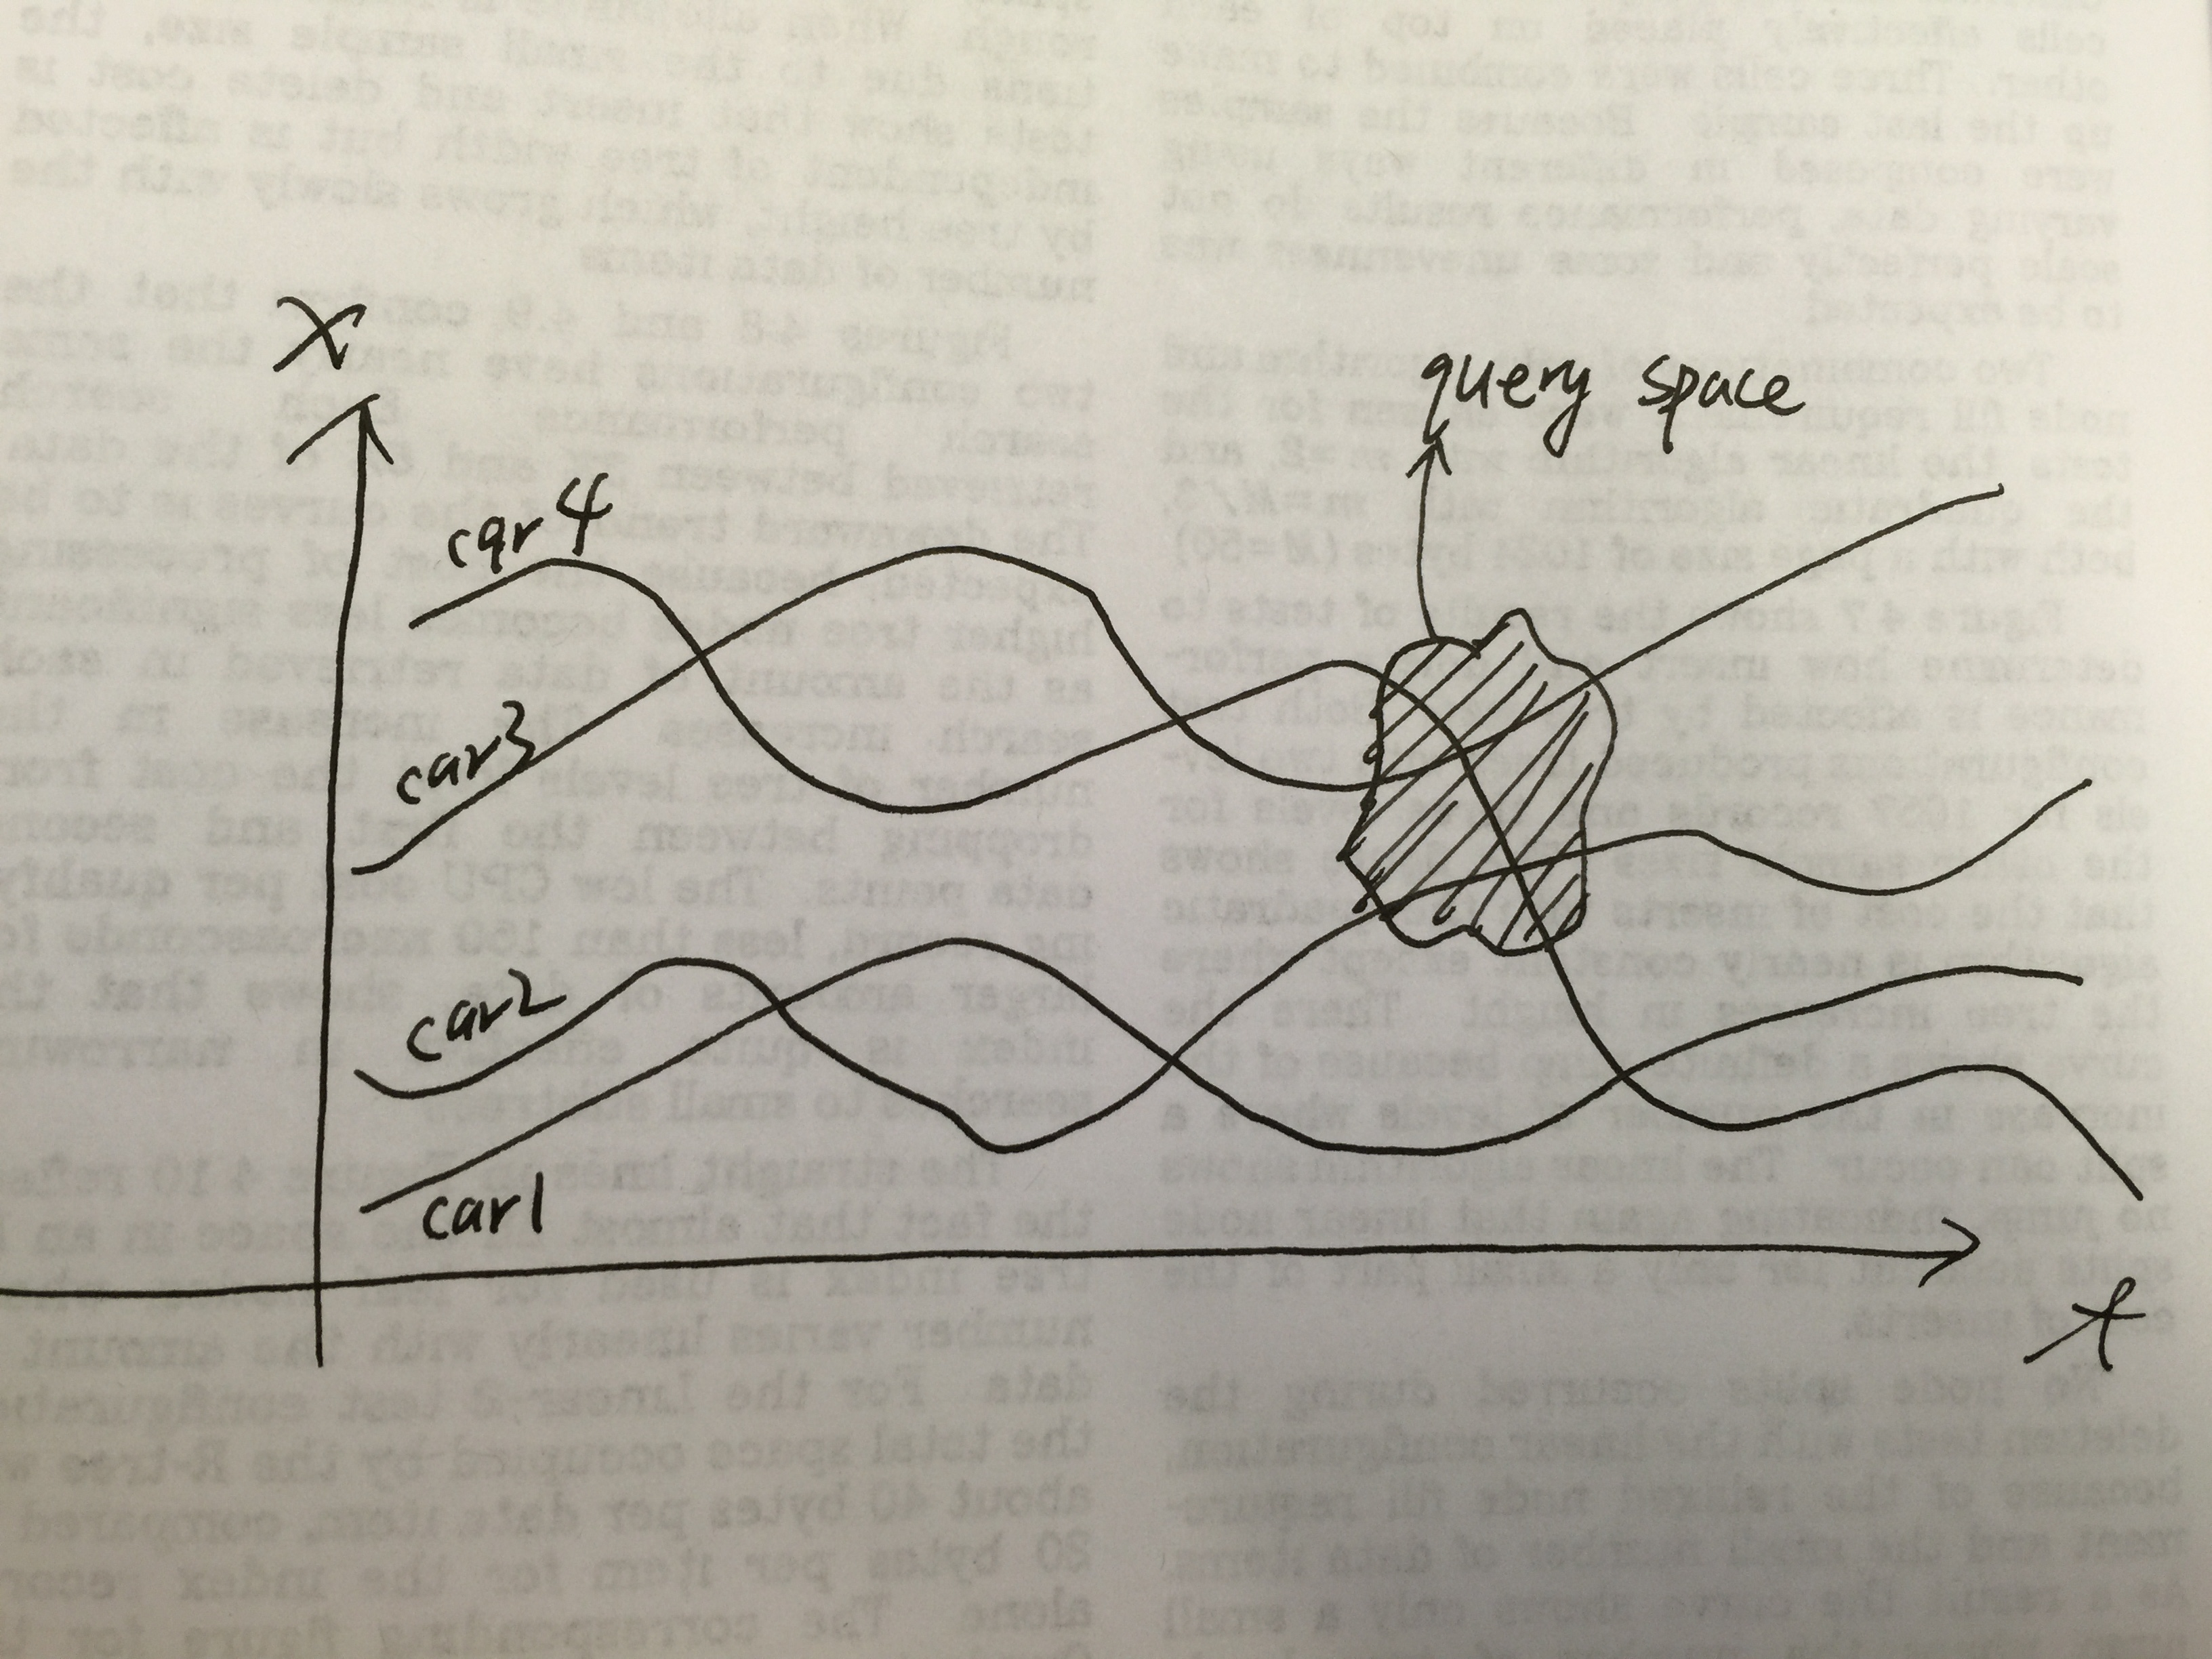
\includegraphics[width=90mm]{p1d.jpg}
  \caption{1 Dimension Scenario \label{p1d}}
\end{figure}

We first consider the problem in 1 dimension.
As in figure \ref{p1d},
we have segmented function $X=f(t)$ for each object.
The query space is a closed shape.
The problem is to find the trajectories that satisfy the query space,
i.e. which trajecotry is overlapped by the closed shape.

\begin{figure}[ht!]
  \centering
  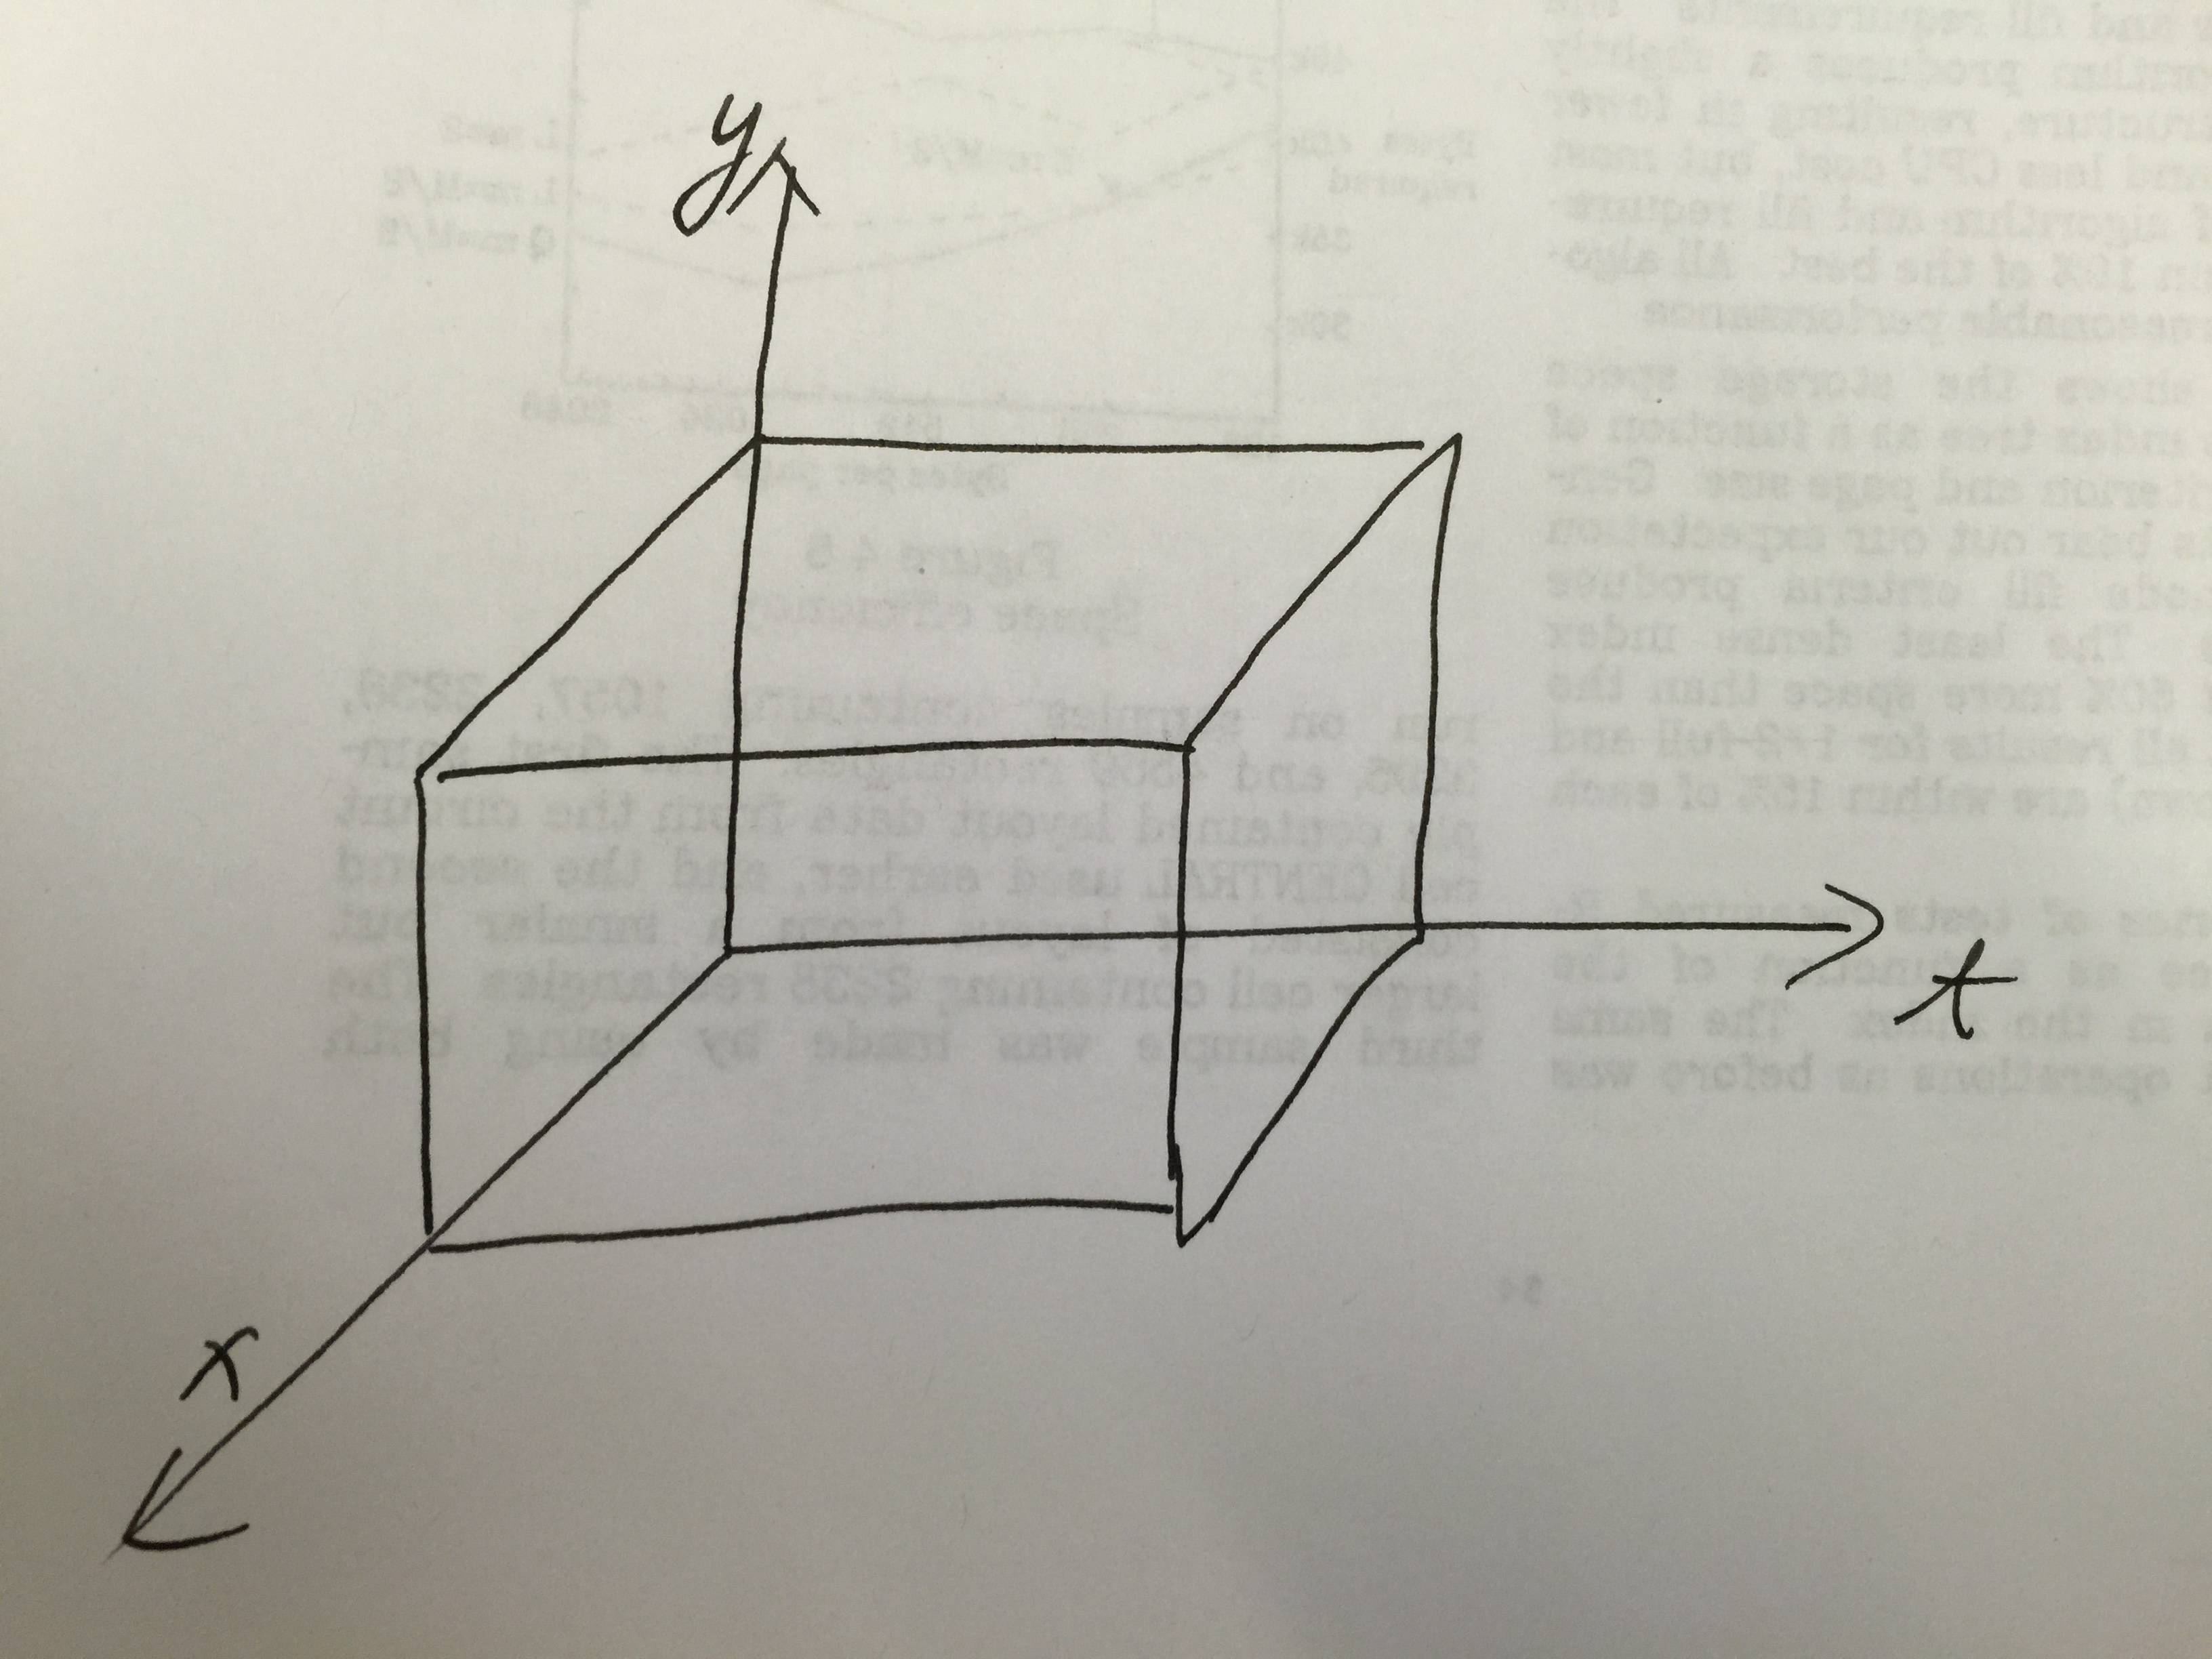
\includegraphics[width=90mm]{p2d.jpg}
  \caption{2 Dimension Scenario \label{p2d}}
\end{figure}

Now we consider the problem in 2 dimension.
As in figure \ref{p2d},
we have segmented function $(x,y) = f(t)$ for each object.
In this scenario, the query space forms a cube.
The problem is similarly to find the trajectories that go through the cube.

Recall that we assume vehicles can only move continuously,
and has a speed limit.
In other words, the car can not jump.

\subsection{Segmented RTree}

\begin{figure}[ht!]
  \centering
  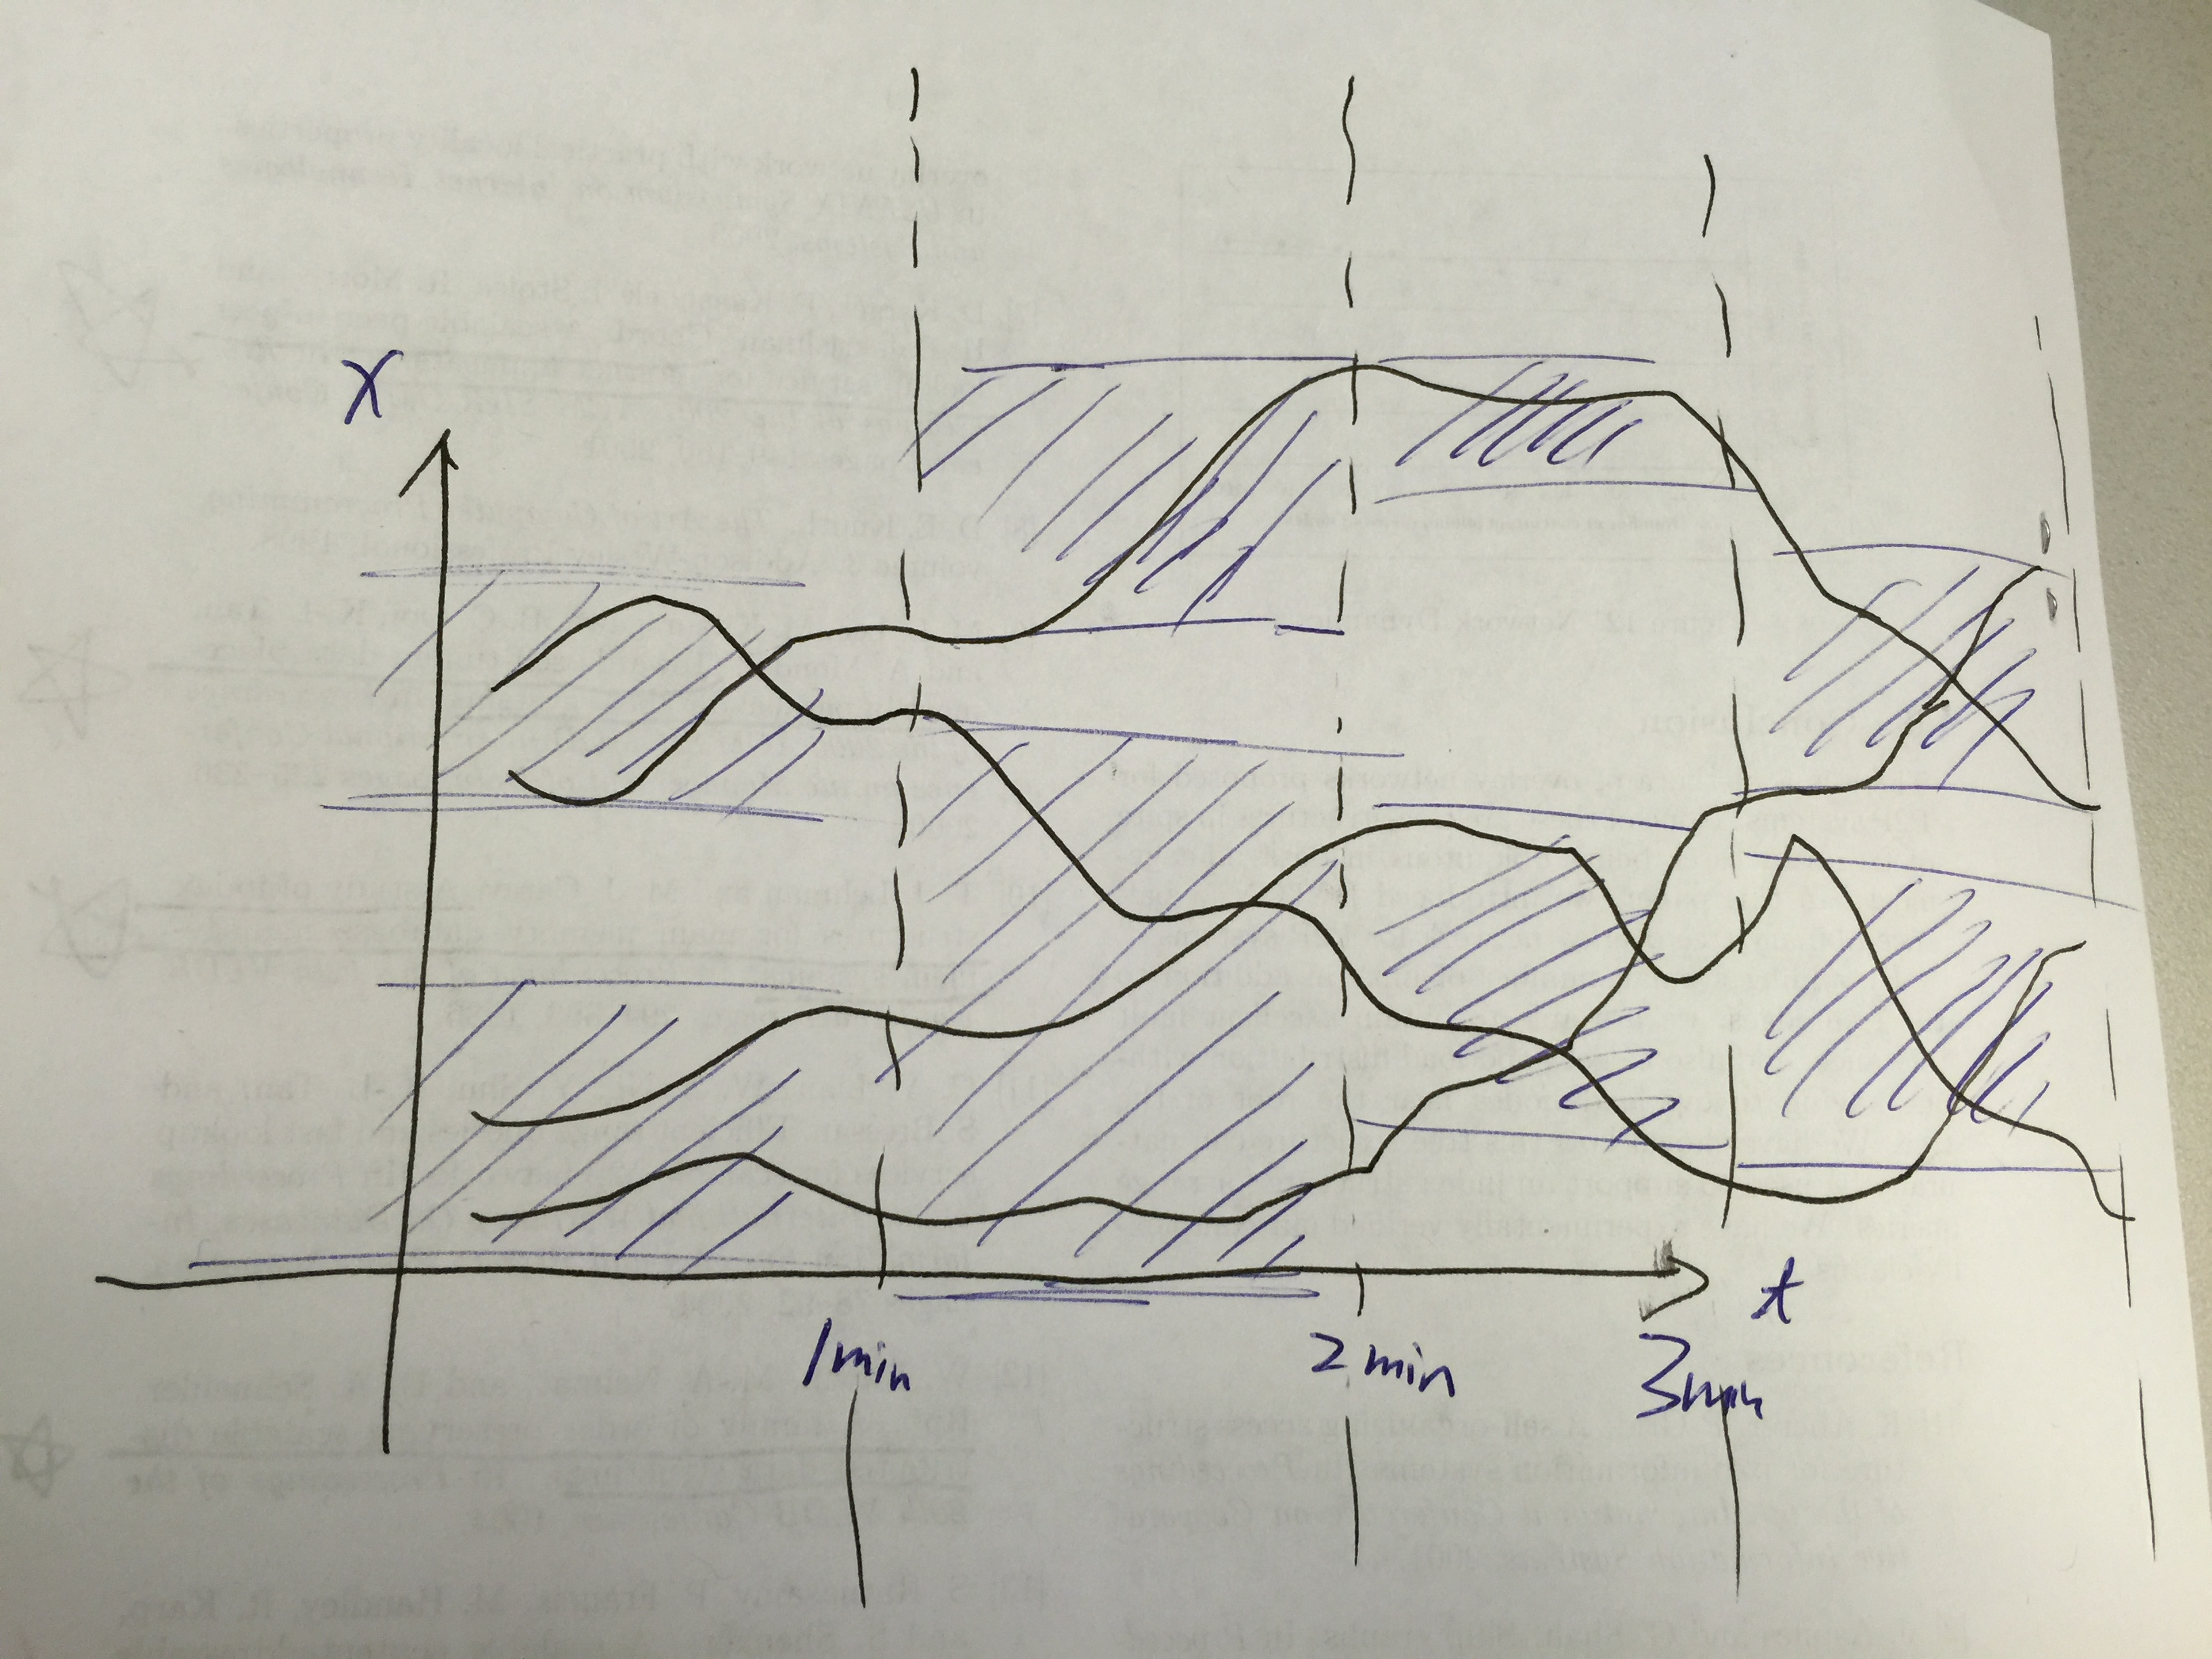
\includegraphics[width=90mm]{seg.jpg}
  \caption{Segmented Trajectory \label{segment_fig}}
\end{figure}

As in figure \ref{segment_fig}, We segment the time dimension into many intervals.
While the whole trajectory of a vehicle can cross a large range of space,
the vechile can only be within a small area in each interval according to our assumption.
Thus we can compute the upper bound and lower bound of the trajectory in each interval.
Then, we build a RTree on every interval to index all vehicles insied this interval.


When the Segmented RTree is built, we can search as follows:
for a given time period, find the overlapped time intervals,
and search the space in RTree on every overlapped intervals.
Synthesize the results together to prepare for the final results.

The problem is tricky to determine what is the appropriate interval length $t_i$.
Thus it became a parameter that can be tuned according to the use case.
When $t_i$ is small, we get more precise on search, because within a smaller time interval,
vehicles will result in smaller area, thus the overlap of vehicles' trajectory will be less.
For example, the vehicles in an area within 5 minutes can be much more than in the same area within 20 seconds.
However, the smaller $t_i$ is, the more segments we will get, and the more RTree will have to be built.
On the other hand, larger $t_i$ can be useful if the computation resource is limit,
because the number of RTrees to be built will drop down together with the intermal's increase.
Also, the robostness of the graph will increase because the whole trajectories are dynamic,
vehicles in the system slightly change their trajectory to pick up people on the way.
While small interval suffers from the RTree being rebuilt,
larger interval can be robust and not affected by slight change.

The parameter should be tuned for tradeoff to fit actual needs.
In our implementation, we found interval to be 5 minutes is reasonable and can get good performance.

\section{Implementation}
\label{implementation}

\section{Discusion}
\label{discussion}

\section{Related Work}
\label{related_work}
\subsection{tranporation algorithm}
\subsection{mobile spatial index}

\section{Conclusion}
\label{conclusion}
In this paper, we consider a future scenario that driverless cars become the major transportation method.
We provide the first definition of this problem,
and give an efficient algorithm to schedule this large amount of cars and user requests.
For the key challenge in our schedule algorithm,
index spatial moving objects which has continous trajectory and whose speed has a limitation,
we propose segmented RTree to efficiently solve this important subproblem of index spatial moving objects.

Future work includes how to provide privacy protection,
since people always don't want to expose their trip.
Besides, driverless cars and control center may not necessary belong to the same company.
There may also be many driverless vehicles companies and control center companies.
So we need verification algorithm for the cars know that the shedule is indeed the optimal.

We believe the transportation system will be much more different than it is today,
and we hope our work can stimulate much more valuable work towards next generation transportation.

\balance

\bibliographystyle{abbrv}
\bibliography{driverless}  % vldb_sample.bib is the name of the Bibliography in this case

\end{document}
